
\begin{section}{Approach}
\label{sec:approach}
In this section we describe the framework for detection of sensor attacks for systems with unknown or changing dynamics and adaptive motion to guarantee vehicle safety to solve Problems \ref{problem1} and \ref{problem2}. We follow the architecture in the block diagrams of Fig. \ref{fig:system_arch} and \ref{fig:det_arch}. 



\begin{figure}[ht!]
\vspace{1pt}
\centering
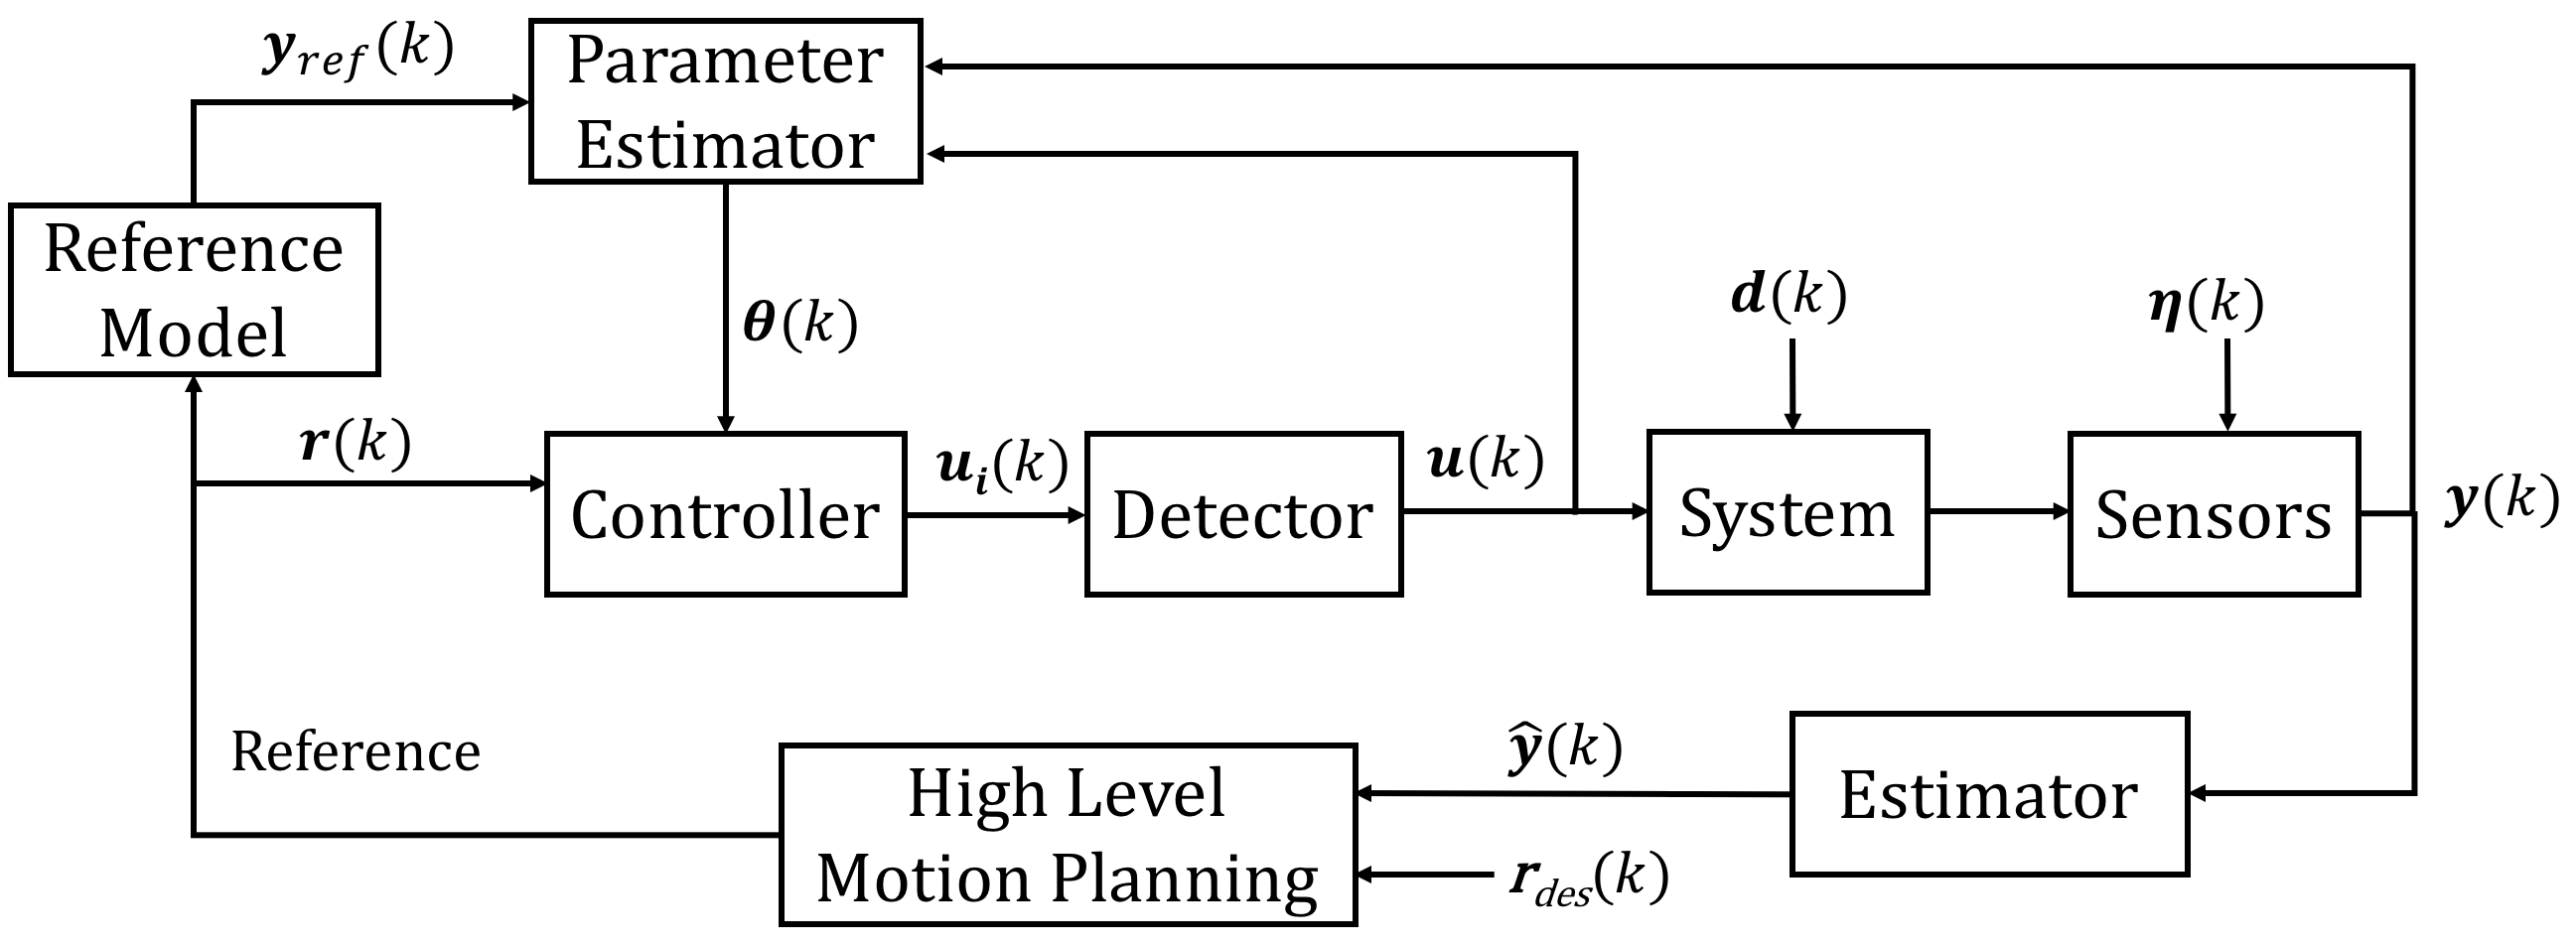
\includegraphics[width=0.48\textwidth]{sys_arch.png}
\caption{Overall system architecture showing the relationship between the reference model adaptive controller and the adaptive motion planner.}
\label{fig:system_arch}
\end{figure}

\subsection{Resilient Adaptive Control}
\label{sec:Res_adapt_control}

The purpose of having model reference adaptive control (MRAC) is to maintain a desired control performance when unknown dynamical changes or disturbances have occurred. Estimation of the system characteristic model's coefficients will help give us this desired performance.
Assumptions for adaptive control: 
	\begin{enumerate}[leftmargin=4\parindent]
	\item[$A1)$] all zeros of $B^{'}(z^{-1})z^m$ are within $|z|<1$. 
	\item[$A2)$] $n$ and $m$ (or their upper bounds) are known. 
	\item[$A3)$] the system delay $d$ is known.
	\end{enumerate}
The objective of model reference adaptive control is to calculate an input signal $u(k)$ such that the system tracks $y^{*}(k)$ given the reference signal $r(k)$. 
A following assumption for the reference model is it satisfies:
    \begin{enumerate}[leftmargin=4\parindent]
	\item[$A4)$] all zeros of $E(z^{-1})z^p$ are within $|z|<1$. 
	\end{enumerate}

The model reference control is designed (Reference to equation!) by solving the polynomial equation:
    \begin{equation}
	E(q^{-1})=F(q^{-1})A(q^{-1})+q^{-d}G(q^{-1})
	\end{equation}
By expressing (Ref to equation $A(q^{-1})y(k)=B(q^{-1})u(k)$) as:
	\begin{equation}
	E(q^{-1})y(k+d)={\alpha}q^{-1}y(k) + {\beta}q^{-1}u(k)=\theta_0^T\phi(k)
	\end{equation}
where,
	\begin{equation}
	\alpha(q^{-1})=G(q^{-1})=\alpha_0+\alpha_1q^{-1}+ \dots +\alpha_{n-1}q^{-n+1}
	\end{equation}
	\begin{align}
	\beta( & q^{-1})=F(q^{-1})B^{'}(q^{-1})=\beta_0+\beta_1q^{-1} \nonumber \\
	& + \dots +\beta_{m+d-1}q^{-m-d+1}, \beta_0\neq0
	\end{align}
we are designing the system to have the same characteristics as the reference model. Parametrization to express this system is:
	\begin{equation}
	\bm{\theta}_0=(\alpha_0, \dots ,\alpha_{n-1},\beta_0, \dots ,\beta_{m+d-1})^T \in R^{n+m+d}
	\end{equation}
	\begin{align}
	\bm{\phi}(j)&=(y(k), \dots ,y(k-n+1),u(k), \dots , \nonumber \\
	& u(k-m-d+1))^T \in R^{n+m+d}
	\end{align}
where $\bm{\theta}_0$ is unknown and $\bm{\phi}(k)$ is known.
	The adaptive control input u(k) is then calculated from the equation:
	\begin{equation}
	\bm{\theta}^T(k)\bm{\phi}(k)=E(q^{-1})y^{*}(k+d)
	\end{equation}
with the equation for the input u(k) as:
	\begin{align}
	u(k)=\frac{1}{\theta_{n+1}(k)}&(-\theta_1(k)y(k)-\theta_2(k)y(k-1)  \nonumber \\
    -\dots-\theta_n(k)y(k&-n-1)-\theta_{n+2}(k)u(k-1)  \\
	-\theta_{n+3}(k)u(k-2)-& \dots - \theta_{n+m+d}(k)u(k-m-d+1) \nonumber \\
	+g&H(q^{-1})r(k))^T \nonumber
	\end{align}
	\begin{equation}
	\bm{\theta}(k)=(\theta_1(k), \dots ,\theta_n(k),\theta_{n+1}(k), \dots ,\theta_{n+m+d}(k))^T
	\end{equation}
where $\bm{\theta}(k)$ is the estimate of the true parameter vector $\bm{\theta}_0$, updated by the modified projection algorithm:
	\begin{equation}
	\bm{\theta}(k)=\bm{\theta}(k-1)+\frac{a(k)\phi(k-d)e(k)}{c+\phi^T(k-d)\phi(k-d)}
	\end{equation}
	\begin{equation}
	\bm{e}(k)=E(q^{-1})y(k)-\theta^T(k-1)\phi(k-d)
	\end{equation}
	\begin{align*}
	\varepsilon<a(k)<2-\varepsilon, 0,\varepsilon<1, c>0
	\end{align*}
To avoid division by $0$, $\theta_{n+1}(k)\neq0$ is necessary.

For detection, model reference adaptive control is an effective solution to the problem of dynamically changing or unknown systems. \cite{tao2003adaptive} states that under the assumptions (A1-A4), it ensures:
	\begin{enumerate}[label=(\roman*),leftmargin=4\parindent]
	\label{assumtions_ensure}
	\item $y(k)$ and $u(k)$ are bounded 
	\item $\lim_{k\to\infty}(y(k)-y^*(k))=0$
	\item $\sum_{k=0}^\infty(y(k)-y^*(k))^2<\infty$
	\end{enumerate}
This states the system's output $y(k)$ will asymptotically converge to the tracking reference signal $y^*(k)$ in a finite amount of time. Properties of the modified projection algorithm include,
    \begin{enumerate}[label=(\roman*),leftmargin=3\parindent]
	\item every iteration improves estimation:
	    \begin{align}
	        \|\bm{\theta}(k)-\bm{\theta}_0\|\leq\|\bm{\theta}(k-1)-\bm{\theta}_0\|\leq\|\bm{\theta}(0)-\bm{\theta}_0\|, k\geq1 \nonumber
	    \end{align}
	\item parameter variation has finite energy:
	    \begin{align}
	        \sum_{k=1}^\infty{\|\bm{\theta}(k)-\bm{\theta}(k-1)\|}^2\leq \infty \nonumber
	    \end{align}
	\item parameter variation converges to zero:
	    \begin{align}
	        \lim_{k\to\infty}(\bm{\theta}(k)-\bm{\theta}(k-1))=0 \nonumber
	    \end{align}
	    \begin{align}
	        \lim_{k\to\infty}(\bm{\theta}(k)-\bm{\theta}(k-N))=0, \text{any finite } N>0 \nonumber
	    \end{align}
	\end{enumerate}

Each system output measurement $\bm{y}_i$ where $i=1,2,\dots,N_y$ and $N_y$ is the total number of outputs to be measured. Every $\bm{y}_i$ output measurement has $j$ number of sensors capable of provided data, represented in the form $\bm{y}_{i,j}$. Each of the sensor measurements $\bm{y}_{i,j}$ providing data of each output experience the same convergence behavior to the tracking signal when the sensors are uncompromised. This remains true with a changing reference signal, changing system dynamics, or bounded disturbances. 
With the assurances of (\ref{assumtions_ensure}), it is true that all uncompromised outputs track its given reference signal via the reference model.
\begin{equation}
\label{multiple_output_tracking}
    \lim_{k\to\infty}(y_{i,j}(k)-y^*_i(k))=0, \text{ }\forall j
\end{equation}
For each $i^{th}$ measured output, a total of $j$ number of MRAC subsystems are built to monitor for dynamical changes and sensor attacks. Each subsystem receives it's own individual $j^{th}$ sensor signal, but they all share the same reference model, reference signal $r(k)$, and input $u_i(k)$ that is directly used to control the vehicle to a desired output. Each MRAC subsystem calculates an updated input $u_{i,j}$ that are fed into the detector, which analyses each $j^{th}$ input-output combination to check for comprised sensors. With (\ref{multiple_output_tracking}) ensured, we can also say:
\begin{equation}
    \lim_{k\to\infty}(u_{i,j}(k)-u_{i,j^*}(k))=0, \text{ }j\neq j^*
\end{equation}
where $j$ and $j^*$ refer to subsystems generating an input to control the same output.

\NB{add Lemma}

\begin{figure}[ht!]
\vspace{1pt}
\centering
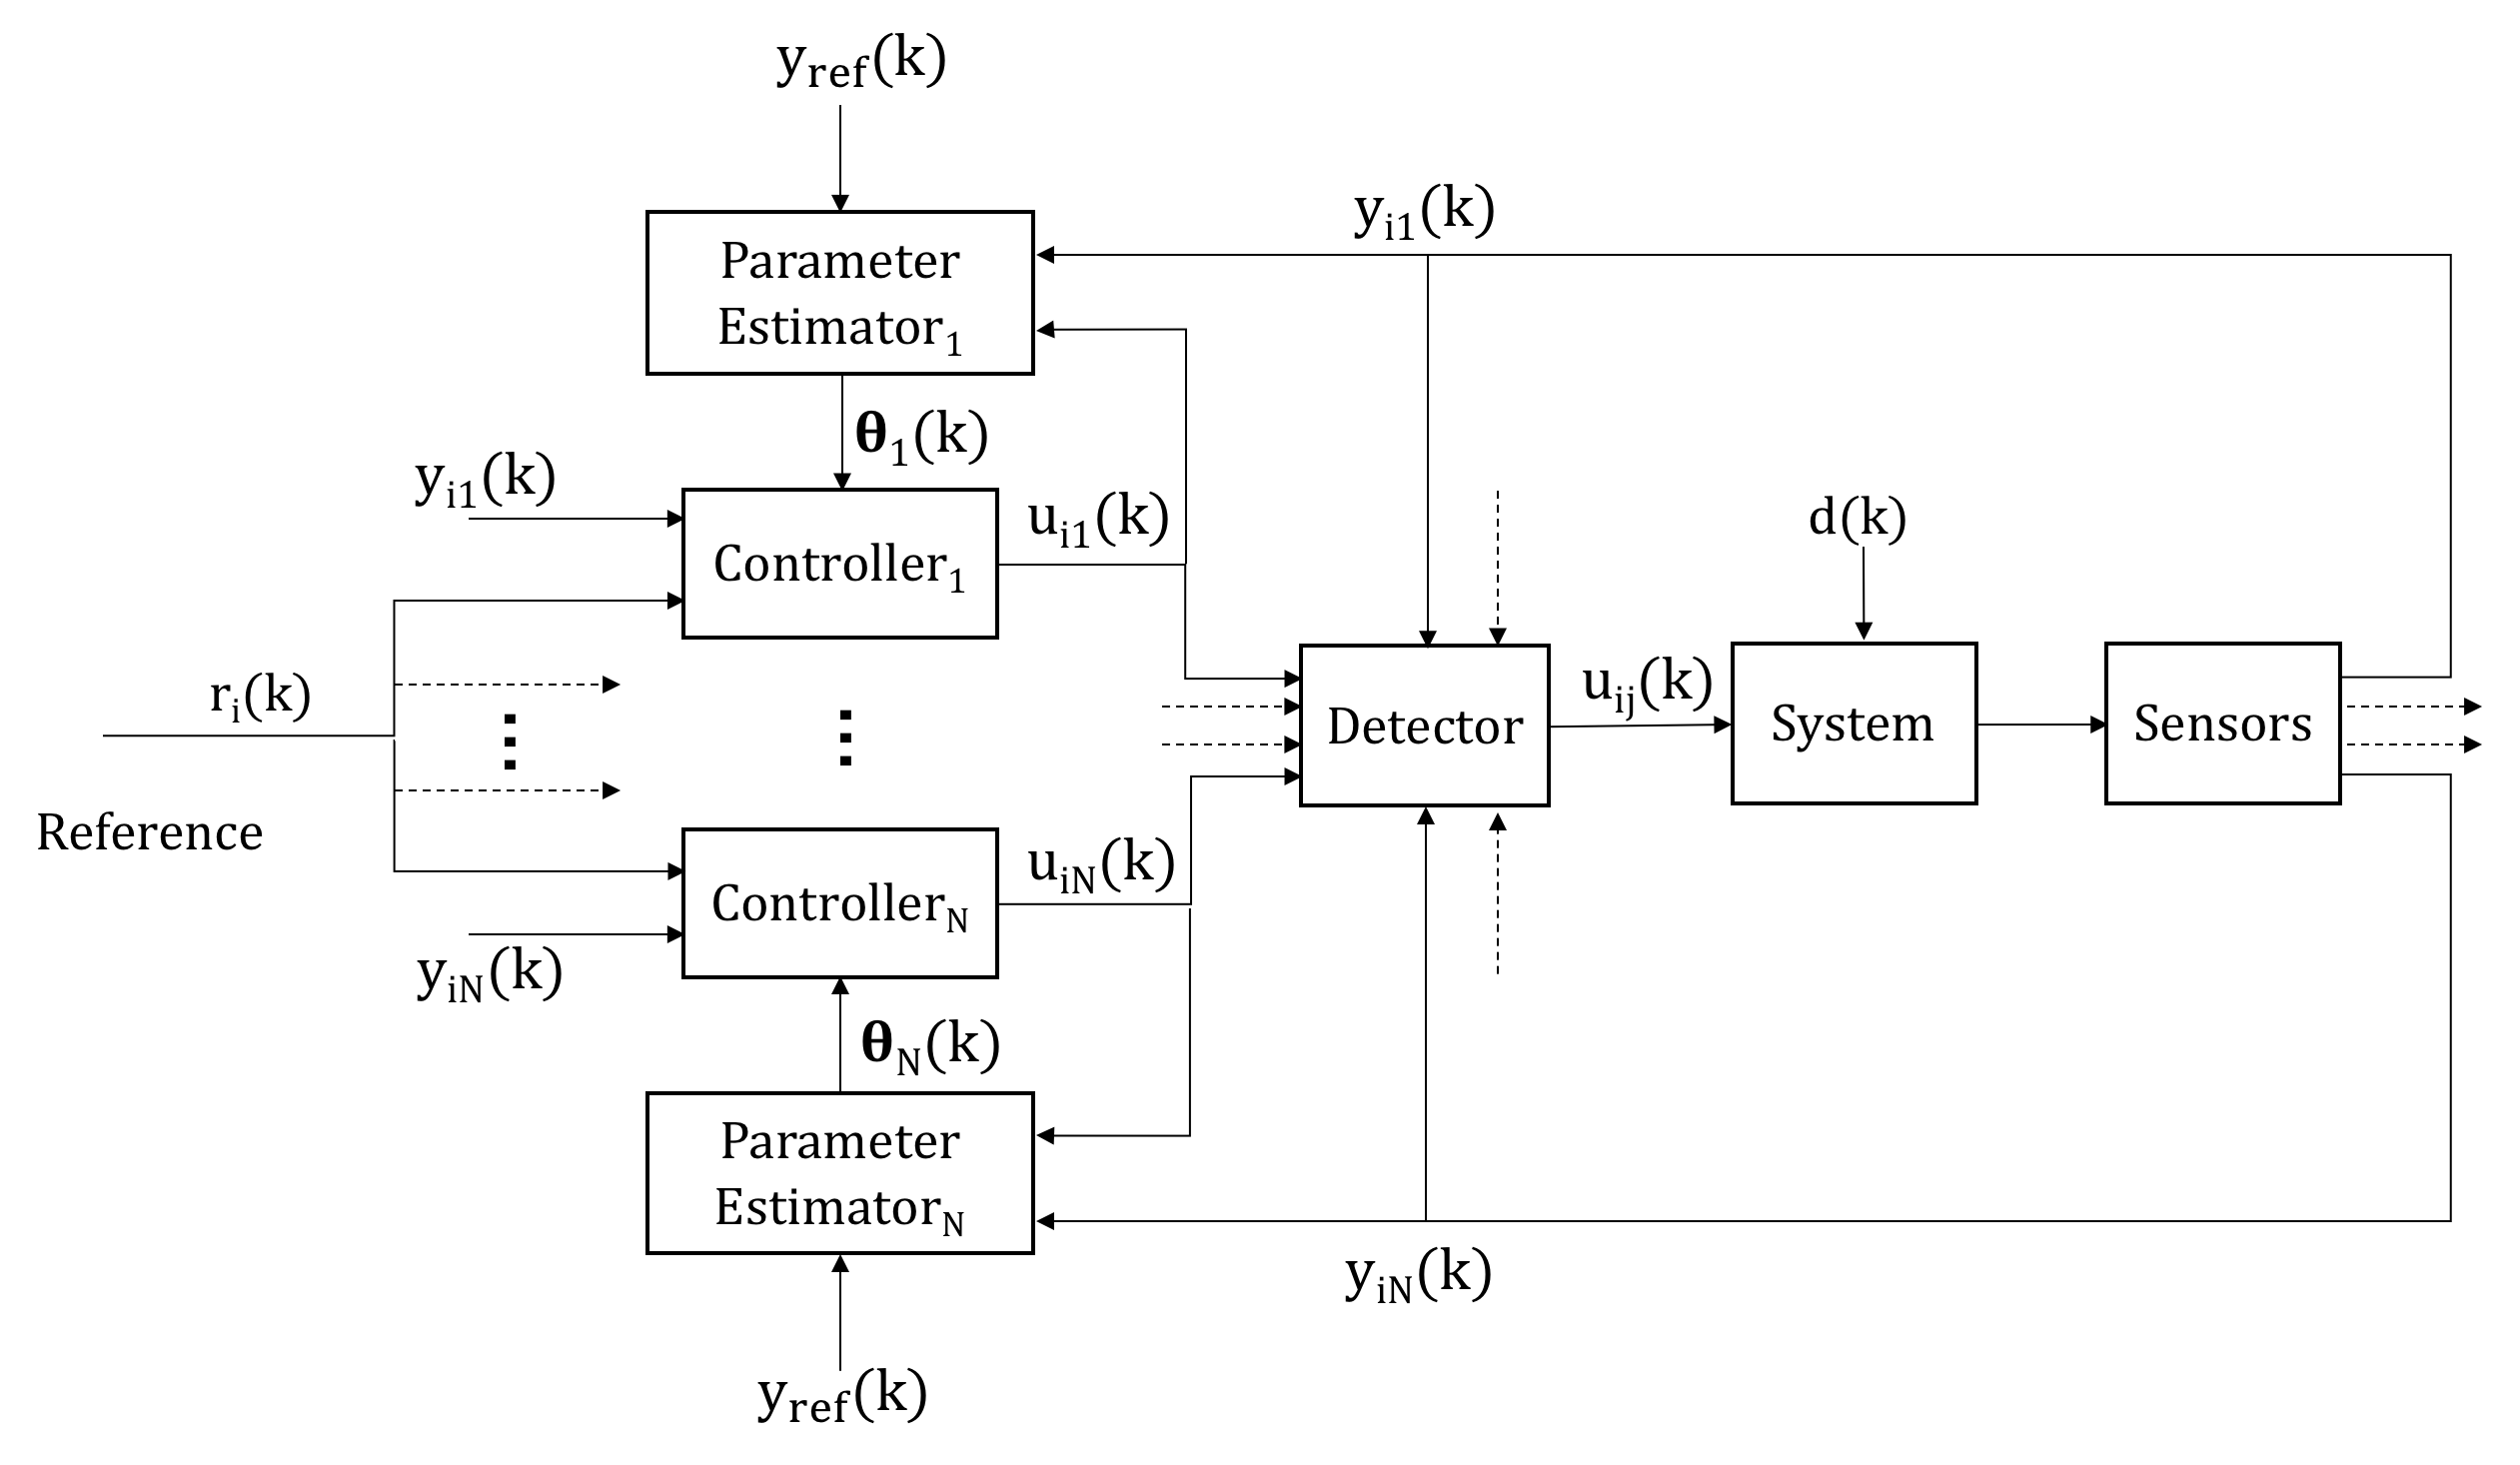
\includegraphics[width=0.48\textwidth]{con_and_det.png}
\caption{System architecture of the detection scheme within the adaptive controller. Representing the $i^{th}$ output state and the $j^{th}$ number of available measurement sensors for that output.}
\label{fig:det_arch}
\end{figure}

When an attacker maliciously falsifies a sensor signal, the $j^{th}$ output sensor measurement of the $i^{th}$ output state no longer follows the converge rate compared to the uncompromised sensor measurements. As the $j^{th}$ sensor of the $i^{th}$ output no longer follows convergence characteristics, it is removed from the set of uncompromised output sensor measurements $\bm{Y}$ to ensure proper control and estimation for navigation safety. The new set of output measurements is defined as $\bm{Y}=\bm{Y}_0-\bm{Y}_a$ where $\bm{Y}_0$ is the initial uncompromised output measurement set and $\bm{Y}_a$ is the set of attacked output sensors that have been removed. Effective detection is constrained to when $\leq \frac{N_i}{2}$ of sensors are attacked, where $N_i$ is the total number of available sensors for the $i^{th}$ output.


%%%%%%%%%%%%%%%%%%%%%%%%%%%%%%%%%%%%%%%%%%%%%%%%%%%%%%%%%

\subsection{Estimation}
For positional estimation with sensor uncertainties, we need a guarantee the vehicle is within a region to prevent navigation into an undesired state. Using an $N$ number of data samples of known variance $\sigma_p^2$, we are able to estimate a region of a specific confidence that the vehicle is within the region's boundaries.
\begin{figure}[ht!]
\vspace{1pt}
\centering
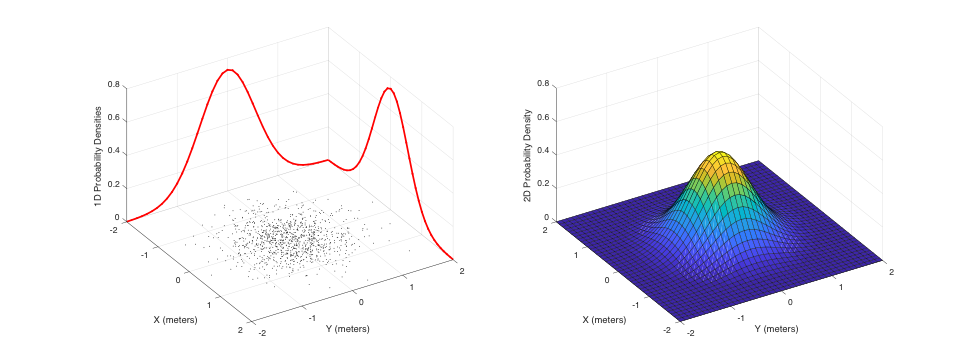
\includegraphics[width=0.48\textwidth]{GaussianPDF.png}
\caption{Distribution of data samples in an $X-Y$ plane with equal noise variance on the $X$ and $Y$ axis.}
\label{fig:gauss_pdf}
\end{figure}
In this work, the statistical technique of confidence intervals is the foundation of how we solve for estimation. Confidence intervals are used to estimate where the true mean lies in a given stochastic sample of data. 
    \begin{equation}
     \label{Confidence_interval}
		C_I = \bar{x} + z^{*}\frac{\sigma}{\sqrt{N}}
	\end{equation}
Assuming the knowledge of the confidence percentage $z^{*}$, population standard deviation $ \sigma $, the number of sensor data samples $N$, and the mean of the sensor data samples $ \bar{x} $, a confidence interval of a chosen percentage can be calculated. As the $N$ number of samples grow, the radius of the confidence interval shrinks giving a better estimation of the true mean with the same confidence level.
% The region $\varepsilon_{x,y|N}$ is described as having the center point at $\bar{y}_{x,y}$ and radius of,

For this paper, this method guarantees the center of the vehicle has a specific percentage of confidence that it's within this region. The data being used for estimation, regardless if it's raw or filtered data, has the form $\mathcal{N}(0,\sigma_p)$ where the data population standard deviation $\sigma_p$ is known for any sensor combination. Using (\ref{Confidence_interval}) we can find a multivariate region of a determined confidence percentage that the vehicle is within to ensure safety:
    \begin{equation}
    \label{Confidence_region}
		\hat{\bm{\varepsilon}}_{x,y|N} = \hat{\bar{y}}_{x,y} + z^{*}\frac{\sigma_p}{\sqrt{N}}
	\end{equation}
Where its radius is,
    \begin{equation}
		\hat{\varepsilon}_r = z^{*}\frac{\sigma_p}{\sqrt{N}}
	\end{equation}
Similar to the calculation of confidence intervals, it is under the assumption that the true mean, or in our case the vehicle, is not changing positions over the $N$ number of sampled data points used in the confidence interval region calculation.

 This cannot be assumed in the case of position estimation of a navigating vehicle. A pseudo-static form of a confidence region is made to compensate for translation of previous position measurements $\bm{y}_{x,y}(k-i)$, where $i=1,2,\dots,N$. These $N-1$ number of previous position data points need to be represented as if they were all sampled for the current position in time $k$, creating a pseudo-static set of data to calculate the confidence region. (SHOW THIS IN A FIGURE FOR BETTER VISUAL UNDERSTANDING, either Matlab or Powerpoint).

The unaltered $N$ data samples are described in two sets,
\begin{equation}
    \mathcal{\bm{X}}=\begin{bmatrix} y_x(k-1) ,y_x(k-2),\dots,y_x(k-N) \end{bmatrix} \nonumber
\end{equation}
\begin{equation}
    \mathcal{\bm{Y}}=\begin{bmatrix} y_y(k-1) ,y_y(k-2),\dots,y_y(k-N) \end{bmatrix} \nonumber
\end{equation}
for the positional coordinate data in the $x$ and $y$ direction. Translating the data coordinates into a pseudo-static form will create the updated sets,
\begin{equation}
    \mathcal{\bm{X}}^*=\begin{bmatrix} y_x^*(k-1) ,y_x^*(k-2),\dots,y_x^*(k-N) \end{bmatrix} \nonumber
\end{equation}
\begin{equation}
    \mathcal{\bm{Y}}^*=\begin{bmatrix} y_y^*(k-1) ,y_y(^*k-2),\dots,y_y^*(k-N) \end{bmatrix} \nonumber
\end{equation}
Each element of these updated sets are calculated as:
    \begin{equation}
	y_x^*(k-i) = y_x(k-i)+\sum_{j=1}^i v(k-j)\cos{\theta_h(k-j)T_s}
	\end{equation}
	\begin{equation}
	y_y^*(k-i) = y_y(k-i)+\sum_{j=1}^i v(k-j)\sin{\theta_h(k-j)T_s}
	\end{equation}
The mean of each set is written as $\hat{\bar{y}}_x^*$ and $\hat{\bar{y}}_y^*$ is used for the calculation of the estimated confidence interval region.

Creating a pseudo-static case with these past position data samples introduces higher uncertainty. Uncertainties regarding the actuator $\sigma_a$, velocity sensor $\sigma_v$, and heading angle sensor $\sigma_h$ need to be accounted for. To guarantee the true position of the vehicle is within the estimation radial bounds, the maximum error in position due to the actuator and sensor noises over the furthest sample in time in $\mathcal{\bm{X}}$ and $\mathcal{\bm{Y}}$ is calculated as:
    \begin{equation}
	\hat{\varepsilon}_{v,\theta_h|N}^{\star}=\sqrt{(v^{\star}\cos{\theta_h^{\star}})^2+(v^{\star}\sin{\theta_h^{\star}})^2}
	\end{equation}
where,
    \begin{equation}
	v^{\star}=\bar{v}(k-i_{\varepsilon^{\star}})+z^{*}\sigma_v \nonumber
	\end{equation}
	\begin{equation}
	\theta_h^{\star}=\bar{\theta}_h(k-i_{\varepsilon^{\star}})+z^{*}\sigma_h \nonumber
	\end{equation}
with $i_{\varepsilon^{\star}}=[1,2,,\dots,N]$ while average measured velocity and average measured heading angles over the past $N$ samples are denoted $\bar{v}$ and $\bar{\theta}_h$, respectively. Doing this will protect the integrity of the confidence interval region, ensuring the vehicle is within its estimation bounds.

\subsection{Adaptive Motion Planning}
With uncertainty of sensor measurements, with or without the loss of a compromised sensors, there needs to be guarantees to safely navigate a vehicle without accidents. As obstacles or unwanted regions approach the vehicle with position uncertainty, changes to the vehicle's motion need to be made. To keep the vehicles estimated confidence region from intersecting with an unwanted region, a change to the number of current and past data samples in the calculation as well as an adaptation of the velocity. With no uncertainty of velocity and heading angle measurements, the equation to solve for the number of required $N$ samples to keep the confidence region within a specific radius is:
    \begin{equation}
    \label{conf_region1}
	    N \geq \left(z^{*} \frac{ \sigma_p }{ {\lVert \bm{x}_{r_{\hat{\bar{y}}}} - \hat{\bar{\bm{y}}}_{x,y}^* \rVert} -\Delta } \right)^2
	\end{equation}
where $\lVert {\bm{x}_{r_{\hat{\bar{y}}}}-\hat{\bar{\bm{y}}}_{x,y}^*} \rVert$ is the distance from the closest undesired region to the estimated vehicle center point position $\hat{\bar{\bm{y}}}_{x,y}^*$.
With the assumption of Normally distributed sensor noise on the velocity and heading angle sensors, the above equation is not suitable. The uncertainty region $\hat{\varepsilon}_{v,\theta_h|(N)}^{\star}$ from these sensors must be accounted for. The revision to equation (\ref{conf_region1}) for a sufficient value of $N$ is:
    \begin{equation}
	    N \geq \left(z^{*} \frac{ \sigma_p }{ {\lVert \bm{x}_{r_{\hat{\bar{y}}}} - \hat{\bar{\bm{y}}}_{x,y}^* \rVert} -[\hat{\varepsilon}_{v,\theta_h|N}^{\star}+\Delta] } \right)^2
	\end{equation}
An update of the reference velocity needs to occur when these undesired regions are within the entire confidence estimation region $ \hat{\varepsilon}_{x,y|N} +\hat{\varepsilon}_{v,\theta_h|N}^{\star}+\Delta$ when $N=1$ to ensure the vehicle slows to capture more previous data samples with less estimation error. This reference velocity $r_v(k)$ update is calculated by:
    \begin{equation}
	    r_v(k)=r_v(k-1) \left[ \frac{\lVert \bm{x}_{r_{\hat{\bar{y}}}} - \hat{\bar{\bm{y}}}_{x,y} \rVert - \hat{\varepsilon}_1}{\hat{\varepsilon}_2 - \hat{\varepsilon}_1} \right]
	\end{equation}
	\begin{equation}
	\begin{split}
	    \hat{\varepsilon}_1=&\hat{\varepsilon}_{x,y|N} +\hat{\varepsilon}_{v,\theta_h|N}^{\star},\\ &\hat{\varepsilon}_2=\hat{\varepsilon}_1+\Delta \nonumber	    
	\end{split}
	\end{equation}
	
where $\hat{\varepsilon}_1$ and $\hat{\varepsilon}_2$ are both radii from the estimated center point $\hat{\bar{\bm{y}}}_{x,y}$.
	
%	\begin{equation}
%		\Delta(k)=[v(k)]^{\delta_v}\delta
%	\end{equation}
%where $[\delta, \delta_v] \in R^{\geq0}$ are chosen values that determine the desired distance between the closest unwanted region to the estimation region as a function of velocity.


% INSERT ALGORITHM FOR REPLANNING VELOCITY
\begin{algorithm}
   \caption{Adaptive Motion for Safe Navigation} 
   \label{alg:adapt_motion} 
    \begin{algorithmic}[1]
	\State Initial conditions of system: $k=0$,$\bm{x}(0)=\bm{x}_0$
	\State Set $r_v(0)$ to desired velocity $r_{v_{des}}(k)$
    \While{$1<k\leq\infty$}
        \State \Longunderstack[l]{ Calculate $\hat{\bar{\bm{y}}}_{x,y}$ then measure closest distance\\ to undesired region $\|\bm{x}_{r_{\hat{\bar{y}}}} - \hat{\bar{\bm{y}}}_{x,y}\|$.}
        \State Calculate radii of intervals $\hat{\varepsilon}_1$ and $\hat{\varepsilon}_2$ for $N$.
        \If{ $\|\bm{x}_{r_{\hat{\bar{y}}}} - \hat{\bar{\bm{y}}}_{x,y}\| < \hat{\varepsilon}_2(k)$}
            \State Solve for suitable $N$ of next iteration
            \State Update reference for velocity $r_v(k)$
        \Else
            \If{$\|\bm{x}_{r_{\hat{\bar{y}}}} - \hat{\bar{\bm{y}}}_{x,y}\| < \varepsilon_2(k)$ when $N=1$}
                \State Solve for a suitable $N$
                \State Update reference for velocity $r_v(k)$
            \Else
                \If{$r_v(k) \neq r_{v_{des}}$}
                    \State Reference velocity $r_v(k)=r_{v_{des}}$
                    \State $N = 1$
                \Else
                    \State Reference velocity $r_v(k) = r_v(k-1)$
                    \State $N = 1$
                \EndIf
            \EndIf
        \EndIf
    \EndWhile
	\end{algorithmic}
\end{algorithm}



\end{section} 